\documentclass[12pt]{jarticle}
\usepackage{TUSIreport}
\usepackage{otf}
\usepackage[dvipdfmx]{graphicx}
\usepackage[dvipdfmx]{color}
\usepackage{amsmath}
\usepackage{amssymb}
\usepackage{color}
\usepackage{hhline}
\usepackage{fancybox,ascmac}
\usepackage{multirow}
\usepackage{url}
\usepackage{bm}
\usepackage{listings,jlisting}
%%%%%%%%%%%%%%%%%%
\lstdefinestyle{py}{
    language={Python},
    backgroundcolor={\color[gray]{.85}},
    basicstyle={\small},
    identifierstyle={\small},
    commentstyle={\small\ttfamily \color[rgb]{0,0.5,0}},
    keywordstyle={\small\bfseries \color[rgb]{1,0,0}},
    ndkeywordstyle={\small},
    stringstyle={\small\ttfamily \color[rgb]{0,0,1}},
    frame={tb},
    breaklines=true,
    columns=[l]{fullflexible},
    numbers=left,
    xrightmargin=0zw,
    xleftmargin=3zw,
    numberstyle={\scriptsize},
    stepnumber=1,
    numbersep=1zw,
    morecomment=[l]{//}
}
\begin{document}
%%%%%%%%%%%%%%%%%%%%%%%%%%%%%%%%%%%%%%%%%%%%%%%%%%%%%%%%
% 表紙を出力する場合は,\提出者と\共同実験者をいれる
% \提出者{科目名}{課題名}{提出年}{提出月}{提出日}{学籍番号}{氏名}
% \共同実験者{一人目}{二人目}{..}{..}{..}{..}{..}{八人目}
%%%%%%%%%%%%%%%%%%%%%%%%%%%%%%%%%%%%%%%%%%%%%%%%%%%%%%%
\提出者{情報工学実験3}{課題4 画像変換}
{2021}{4}{29}{4619055}{辰川力駆}
%%%%%%%%%%%%%%%%%%%%%%%%%%%%%%%%%%%%%%%%%%%%%%%%%%%%%%%%%
\共同実験者{}{}{}{}{}{}{}{}
%%%%%%%%%%%%%%%%%%%%%%%%%%%%%%%%%%%%%%%%%%%%%%%%%%%%%%%%%
% 表紙を出力する場合はコメントアウトしない
%%%%%%%%%%%%%%%%%%%%%%%%%%%%%%%%%%%%%%%%%%%%%%%%%%%%%%%%%
\表紙出力
%%%%%%%%%%%%%%%%%%%%%%%%%%%%%%%%%%%%%%%%%%%%%%%%%%%%%%%
% 以下はレポート本体,reportmain.tex に書いてある.
% \inputを使っているが,直接書いても良い.
%%%%%%%%%%%%%%%%%%%%%%%%%%%%%%%%%%%%%%%%%%%%%%%%%%%%%%%
\section{実験の要旨}

畳み込み演算を用いた画像変換を実装して高速化し、
グラフを用いて速度を比較する。

\section{実験の目的}

画像変換の処理を題材に、
画像処理のプログラミングと評価を通じて、
画像処理の基本的な考え方を理解することを目的とする。

第2回目の実験では、
畳み込み演算を用いた画像変換を実装することで空間フィルタリングについて理解することを目的とする。

\section{課題1}
\subsection{実験方法}

himeji\_noise.pngを用いて平均化フィルタを実装する。
\begin{figure}[h]
    \begin{center}
        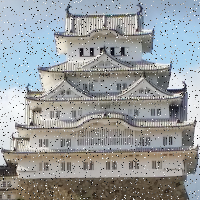
\includegraphics[scale=0.7]{kadai4_2_3.png}
    \end{center}
    \caption{himeji\_noise.png}
\end{figure}

\begin{enumerate}
    \item OpenCV、scikit-image等のライブラリを使用せずに、
          pythonとnumpyのみを用いて平均化フィルタ myaverage\_naive(image, size) を実装する。

    \item scikit-imageを用いて実装した平均化フィルタと結果が一致することを確認する。
          (平均二乗誤差$\mbox{MSE}$が1未満であることを確認する。)

    \item 積分画像(integral image)を用いて平均化フィルタを高速化した myaverage\_integral(image, filter\_size) を実装し、
          2と同じようにscikit-imageによる平均化フィルタの処理結果と一致することを確認する。

    \item 画像サイズを変化させながら、2つのフィルタ関数 myaverage\_naive()、 myaverage\_integral() の処理時間を計測し、
          グラフを描いて比較するとともに、計算量の観点から考察する。
    \item フィルタサイズを変化させながら、2つのフィルタ関数 myaverage\_naive()、myaverage\_integral() の処理時間を計測し、
          グラフを描いて比較するとともに、計算量の観点から考察する。
\end{enumerate}

\subsection{実験結果}

作成したプログラムは付録のソースコード1に載せた。
このプログラムを実行して、
scikit-imageを用いて実装した平均化フィルタとのMSEは、
\begin{eqnarray*}
    \text{MSE(naive)} &\approx& 3.178 \times 10^{-28} \\
    \text{MSE(integral)} &\approx& 9.316 \times 10^{-21}
\end{eqnarray*}
となった。つまり、MSEが1未満なので、
scikit-imageを用いて実装した平均化フィルタと結果が一致することがわかる。

また myaverage\_naive()、 myaverage\_integral() において画像サイズを変更したグラフを図2に示した。
さらに myaverage\_naive()、 myaverage\_integral() においてフィルタサイズを変更したグラフを図3に示した。
\begin{figure}[h]
    \begin{center}
        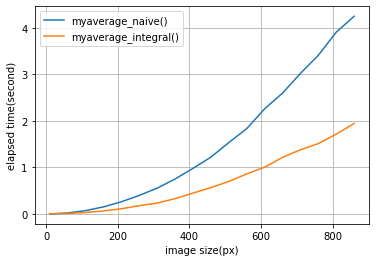
\includegraphics[scale=0.7]{kadai4_2_1.png}
    \end{center}
    \caption{画像サイズを変化した結果}
\end{figure}

\begin{figure}[h]
    \begin{center}
        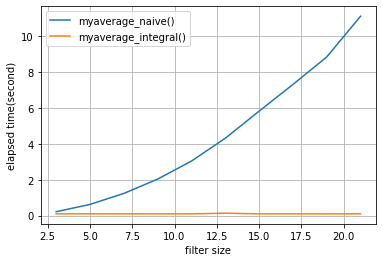
\includegraphics[scale=0.7]{kadai4_2_2.png}
    \end{center}
    \caption{フィルタサイズを変化した結果}
\end{figure}

\clearpage
\subsection{検討・考察}
実験結果の図2,3より、
myaverage\_integral() は、myaverage\_naive() より処理速度が速い。
これを計算量の観点から考える。

myaverage\_naive() は、画像の高さ(px)$\times$幅(px)$\times$ フィルタサイズ $\times$ フィルタサイズ
であるから、O($n^4$)である。
それに対し、myaverage\_integral() は、画像の高さ(px)$\times$幅(px)のみなので、O($n^2$)である。
これは挿入ソートやバブルソートなどの遅めのソートに匹敵する。

よって、積分画像の平均化フィルタの方が高速化できていることが計算量の観点からも分かる。
図3において、myaverage\_integral()がフィルタサイズの影響をあまり受けてない理由も同様である。

\section{まとめ}
本実験では、
畳み込み演算を用いて画像変換を実装し、
空間フィルタリングについて理解することができた。
また、課題では畳み込み演算を行う時とそうでない時とで
どれくらいの速度が違うのかをグラフで考察し、畳み込み演算の有用性について学んだ。


\clearpage
\appendix
\section{付録}

\begin{lstlisting}[style = py,caption=kadai1]
    #4619055
    import time
    import numpy as np
    from skimage.io import imread, imsave
    from skimage.color import rgb2gray, gray2rgb
    from skimage.transform import resize
    from scipy.ndimage.filters import convolve, correlate
    import skimage.transform
    import matplotlib.pyplot as plt
    %matplotlib inline
    
    def mse(y1, y2):
        return ((y1 - y2)**2).mean()
    
    def myaverage_naive(im, filter_size = 5):
        ''' im : 入力画像, filter_size : 平均化フィルタのサイズ(奇数) '''
        iheight, iwidth = im.shape[:2]
        imout = np.zeros((iheight, iwidth))
        
        # ここにコードを追加
        filter = np.ones((filter_size, filter_size)) / (filter_size ** 2)
        im_pad = np.pad(im, (filter_size//2, filter_size//2), mode="constant")
        
        for x in range(filter_size):
            for y in range(filter_size):
                for height in range(iheight):
                    for width in range(iwidth):
                        imout[height, width] += filter[y, x]*im_pad[y+height, x+width]
        
        return imout
    
    def myaverage_integral(im, filter_size = 5):
        ''' im : 入力画像, filter_size : 平均化フィルタのサイズ(奇数) '''
            
        def integral_image(im,pad):
            ''' 積分画像の作成自分で実装 '''
            s = np.zeros_like(im)
            iheight, iwidth = im.shape[:2]
            # 自分で積分画像を求める関数を実装する場合はここにコードを追加
            for i in range(pad+1,iwidth):
                for j in range(pad+1,iheight):
                    s[j, i] = s[j, i - 1] + s[j - 1, i] - s[j - 1, i - 1] + im[j, i]
            return s
        
        iheight, iwidth = im.shape[:2]
        imout = np.zeros((iheight, iwidth))
    
        # ここにコードを追加
        pad = filter_size//2
        im_pad = np.pad(im, ([pad+1, pad], [pad+1, pad]), mode="constant") 
        im_integral = integral_image(im_pad,pad)
        
        for i in range(pad+1, iwidth+pad+1):
            for j in range(pad+1, iheight+pad+1): 
                imout[j-pad-1, i-pad-1] = (im_integral[j+pad, i+pad] - im_integral[j-pad-1, i+pad] - im_integral[j+pad, i-pad-1] + im_integral[j-pad-1, i-pad-1]) / filter_size ** 2
        return imout
    
    def myaverage_separable(im, filter_size):
        ''' im : 入力画像, filter_size : 平均化フィルタのサイズ(奇数) '''
        iheight, iwidth = im.shape[:2]
        imout = np.zeros((iheight, iwidth))
    
        # ここにコードを追加
       
        return imout
    
    im = 255 * rgb2gray(imread("data/himeji_noise.png"))
    filter_size = 3
    
    kernel = np.ones((filter_size, filter_size)) / (filter_size ** 2)
    im2a = myaverage_naive(im, filter_size)
    im2b = myaverage_integral(im, filter_size)
    im2c = myaverage_separable(im, filter_size)   # オプション
    im2_gt = correlate(im, kernel, mode="constant")
    
    print("mse_naive=", mse(im2_gt, im2a))         # 1未満であればOK
    print("mse_integral=", mse(im2_gt, im2b))      # 1未満であればOK
    print("mse_separable=", mse(im2_gt, im2c))     # オプション
    
    #グラフのため
    time_naive_image = []
    time_integral_image = []
    time_naive_filter = []
    time_integral_filter = []
    
    filter_size = 3
    for i in range(10, 900, 50):
        im = 255 * rgb2gray(imread("data/himeji_noise.png"))
        im = skimage.transform.resize(im, (i, i))
        
        elapsed_time = time.time()
        im2a = myaverage_naive(im, filter_size)
        time_naive_image.append(time.time() - elapsed_time)
        
        elapsed_time = time.time()
        im2b = myaverage_integral(im, filter_size)
        time_integral_image.append(time.time() - elapsed_time)
    
    for i in range (3,22,2):
        filter_size = i
        im = 255 * rgb2gray(imread("data/himeji_noise.png"))
        
        elapsed_time = time.time()
        im2a = myaverage_naive(im, filter_size)
        time_naive_filter.append(time.time() - elapsed_time)
        
        elapsed_time = time.time()
        im2b = myaverage_integral(im, filter_size)
        time_integral_filter.append(time.time() - elapsed_time)
        
    plt.plot(range(10,900,50),time_naive_image,label="myaverage_naive()")
    plt.plot(range(10,900,50),time_integral_image,label="myaverage_integral()")
    
    plt.xlabel("image size(px)")
    plt.ylabel("elapsed time(second)")
    plt.grid()
    plt.legend()
    plt.show()
    
    plt.plot(range(3, 22, 2), time_naive_filter, label="myaverage_naive()")
    plt.plot(range(3, 22, 2), time_integral_filter, label="myaverage_integral()")
    
    plt.xlabel("filter size")
    plt.ylabel("elapsed time(second)")
    plt.grid()
    plt.legend()
    plt.show()
\end{lstlisting}


%%%%%%%%%%%%%%%%%%%%%%%%%%%%%%%%%%%%%%%%%%%%%%%%%%%%%%%
\end{document}